\documentclass[11pt, a4paper]{article} %or article has only section and below, book and report also have chapter: http://texblog.org/2007/07/09/documentclassbook-report-article-or-letter/

\usepackage[utf8]{inputenc}  % use utf8 encoding of symbols such as umlaute for maximal compatibility across platforms

\usepackage{caption}    		% provides commands for handling caption sizes etc.
%\usepackage[a4paper, left=25mm, right=20mm, top=25mm, bottom=20mm]{geometry}		 % to easily change margin widths: https://www.sharelatex.com/learn/Page_size_and_margins

\usepackage{etoolbox}    % for conditional evaluations!
%\usepackage{fancyverb}   % for syntax highlighting of R code, together with the listings package
\usepackage[bottom]{footmisc}  % I love footnotes! And they should be down at the bottom of the page!
\usepackage{graphicx}        % when using figures and alike
\usepackage[hidelinks]{hyperref}		% for hyperreferences (links within the document: references, figures, tables, citations)
%\usepackage{listings}

\usepackage{euler}     % a math font, only for equations and alike; call BEFORE changing the main font; alternatives: mathptmx, fourier, 
%\usepackage{gentium} % for a different font; you can also try: cantarell, charter, libertine, gentium, bera, ... http://tex.stackexchange.com/questions/59403/what-font-packages-are-installed-in-tex-live

%------------------------------------------------------------------------------------------------------
%------- text size settings --------------
\setlength{\textwidth}{16cm}% 
\setlength{\textheight}{25cm} %23 
%(these values were used to fill the page more fully and thus reduce the number of pages!)
\setlength{\topmargin}{-1.5cm} %0
\setlength{\footskip}{1cm} %
%\setlength{\hoffset}{0cm} %
\setlength{\oddsidemargin}{1cm}%
\setlength{\evensidemargin}{-.5cm}%
\setlength{\parskip}{0cm} % Abstand zwischen Absätzen
% ----------------------------------------------------------------
\renewcommand{\textfraction}{0.1} % allows more space to graphics in float
\renewcommand{\topfraction}{0.85}
%\renewcommand{\bottomfraction}{0.65}
\renewcommand{\floatpagefraction}{0.70}


\frenchspacing %http://texwelt.de/wissen/fragen/1154/was-ist-french-spacing-was-macht-frenchspacing
%------------------------------------------------------------------------------------------------------
%------------------------------------------------------------------------------------------------------

\usepackage{Sweave}
\begin{document}
%%%%%%%%%%%%% this bit is new to Sweave: %%%%%%%%%%%%%%%%%%%%%  
\Sconcordance{concordance:sweave_document_TB.tex:sweave_document_TB.Rnw:%
<<<<<<< Updated upstream
1 39 1 1 0 22 1 1 8 4 1 1 7 1 2 9 1 2 2 4 1 1 4 1 1 1 4 20 1}
=======
1 39 1 1 0 24 1 1 7 1 2 6 1 1 4 1 2 3 1}
>>>>>>> Stashed changes



\title{Appendix}

\author{Torfinn and Carolina}

\maketitle

%------------------------------------------------------------------------------------------------------
%------------------------------------------------------------------------------------------------------


\section{Introduction}%------------------------------------------------------------------------------------------------------

We created an appendix of meta-analysis paper. To be able to visualize the output, we used an example dataset taken from Gibson et al. 2011.

The dataset to be working with should be named ``data.sub''. The conducted analysis using the function rma from the metafor pacakge should be renamed as such: rma of a random effects model should be named ``rma.RE'' and an rma of a fixed effects model should be named ``rma.FE'' in order for the automatisation to work. IF a meta-regression has been conducted, it should be called ``rma.RE.meta'' or ``rma.FE.meta'' respectively. Other than that, the metafor package in R needs to be installed.  

For creating an appendix with an unkown dataset... \\



\begin{figure}
\captionsetup{width=0.6\textwidth}
\centering
<<<<<<< Updated upstream
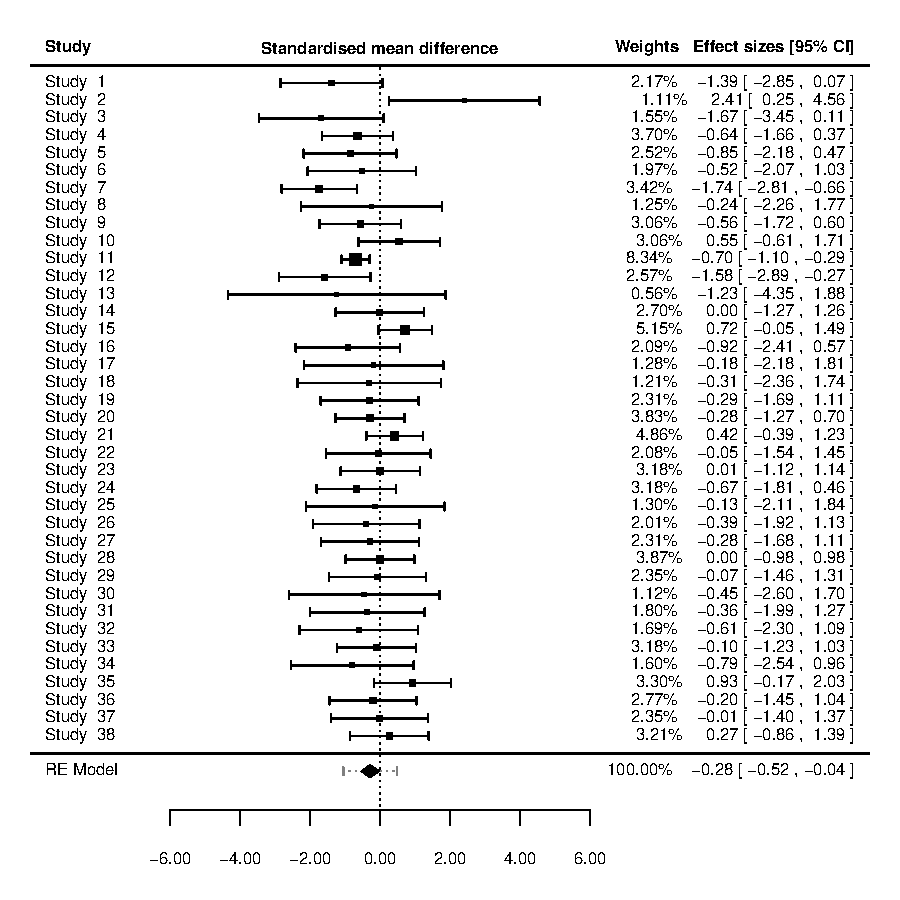
\includegraphics{sweave_document_TB-forest_re}

\caption{Forest plot of a random effects model. The column on the left represents the study. The weighted percentage is shown as well as the effect size (ES) [+- 95\% CI]}
=======
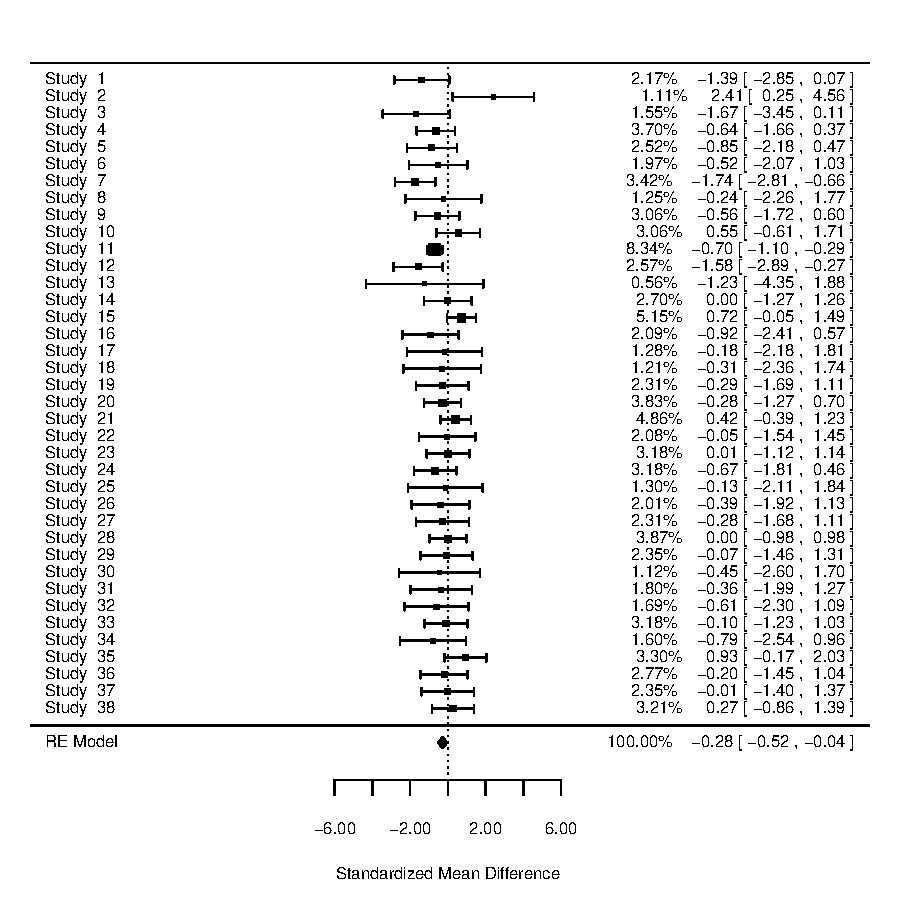
\includegraphics{sweave_document_TB-forestplot}
\caption{Forest plot of a random effects model}
>>>>>>> Stashed changes
\end{figure}


To assess possible publication bias, funnel plots can be used for visualization purposes.

\begin{figure}
\captionsetup{width=0.6\textwidth}
\centering
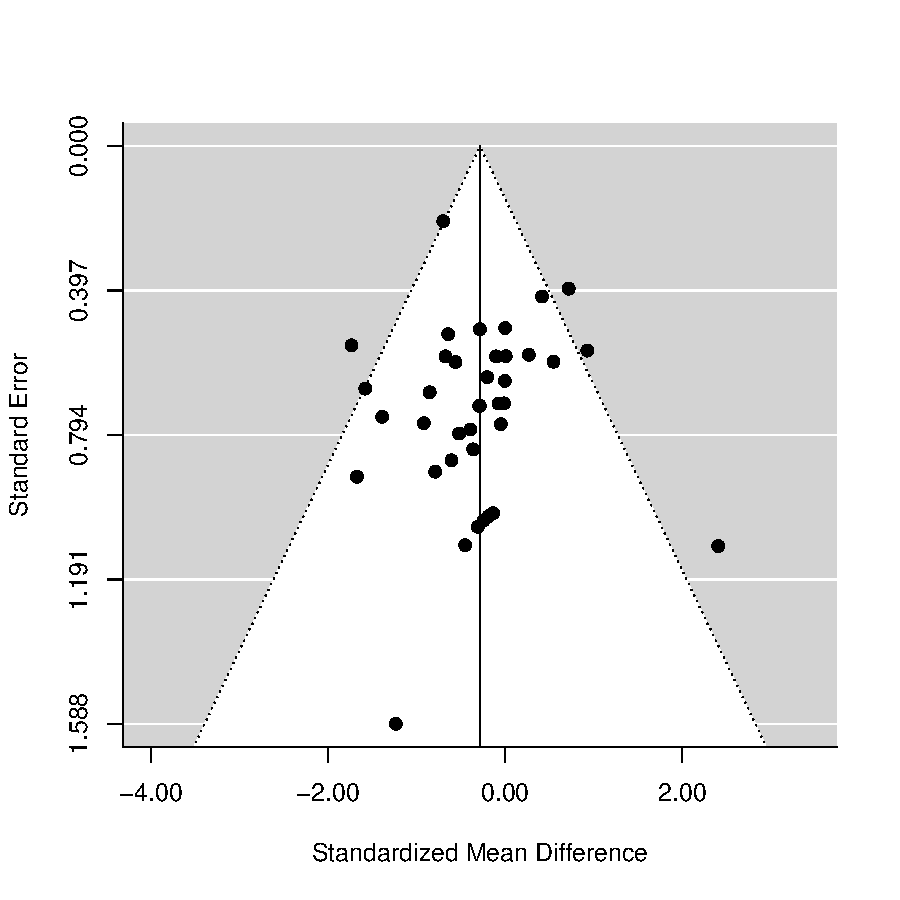
\includegraphics{sweave_document_TB-funnelplot}
<<<<<<< Updated upstream
\caption{Funnel plot of random effects model displaying possible publication bias. The true ES is displayed by the solid verical line.}
\end{figure}


%Should go into the table

%should also go into the table


%% Trying to create a table from rma.RE. Once created, can then specify which parts to keep and with parts not to

%<<echo = FALSE, eval = FALSE>>=
%matrix.RE = data.matrix(rma.RE, rownames.force = NA)
%@

%<<matrix.RE>>=
%require(xtable)
%mytable = matrix.RE
%@

%<<xtable1, results = tex>>=
%xtab = xtable(mytable)
%print(xtab, floating = FALSE)
%@



=======
\caption{Funnel plot that displays possible publication bias}
\end{figure}

>>>>>>> Stashed changes
\end{document}
